\documentclass[../main.tex]{subfiles}
\begin{document}
\section{决策树学习}

\subsection{决策树的概念}
\begin{enumerate}
    \item \textbf{分类（Classification）：}是通过学习获得一个目标函数$f$, 将每个属性集$x$映射到一个预先定义好的类标号$y$\footnote{区分分类与回归：分类目标属性y是离散的，回归目标属性y是连续的}。
    \\解决分类问题的一般方法：模型构建（归纳）、预测应用（推论）。
    \item \textbf{决策树表示法：}内部节点（包括根节点）是属性；节点的后继分支对应该属性的一个可能值；叶子节点是该实例所属分类；决策树代表实例属性值约束的\textbf{合取的析取式}\footnote{意思是说，比如最终分类为“苹果”，那么其实也不止一条路径可以最终分类为苹果，他们之间是“或”的关系，满足其中一条就是苹果了，所以是“析取”；而后，对于每一条路径，其上的所有属性要同时满足才能走过来，所以是“合取”，总而言之就是先每条路径内部合取，然后再不同路径析取}。
    \begin{figure}[H]
        \centering
        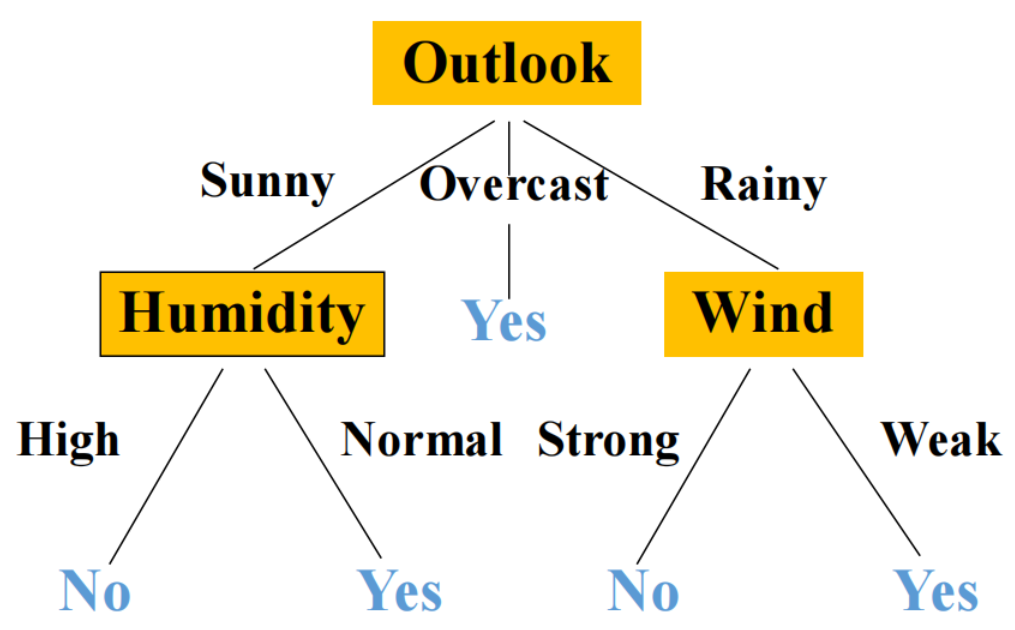
\includegraphics[width=0.55\linewidth]{images/playtennis.png}
        \caption{play tennis的决策树}
        \label{fig:placeholder}
    \end{figure}
    \item{适用问题特征：}“属性-值”对、目标函数离散输出、可能需要析取的描述、训练数据可以包含错误、训练数据可以包含缺少属性值的实例
\end{enumerate}


\subsection{ID3算法}
\begin{enumerate}
    \item \textbf{方法：}采用自顶向下的\textbf{贪婪搜索}遍历可能的决策树空间，使用\textbf{信息增益度}选择测试属性。
    \item \textbf{核心问题：}选取在树的每个节点要测试的属性。
    \item \textbf{熵 (entropy)：}熵表示事物不确定性的程度，也就是信息量的大小\footnote{一般说信息量大,就是指这个时候背后的不确定因素太多，例如小明没有复习裸考人机，却拿到了满绩，背后有很大的信息量，熵就大})，公式如下\footnote{当Entropy最大为1的时候，是分类效果最差的状态，当它最小为0的时候，是完全分类的状态。因为熵等于零是理想状态，一般实际情况下，熵介于0和1之间 。}:
    $$\text{Entropy }=  - \mathop{\sum }\limits_{{i = 1}}^{n}p\left( {x}_{i}\right)  * {\log }_{2}p\left( {x}_{i}\right)$$
    其中, $p\left( {x}_{i}\right)$ 是分类 ${x}_{i}$ 出现的概率，n是分类的数目。可以看出，熵的大小只和变量的概率分布有关。
    \begin{figure}[H]
        \centering
        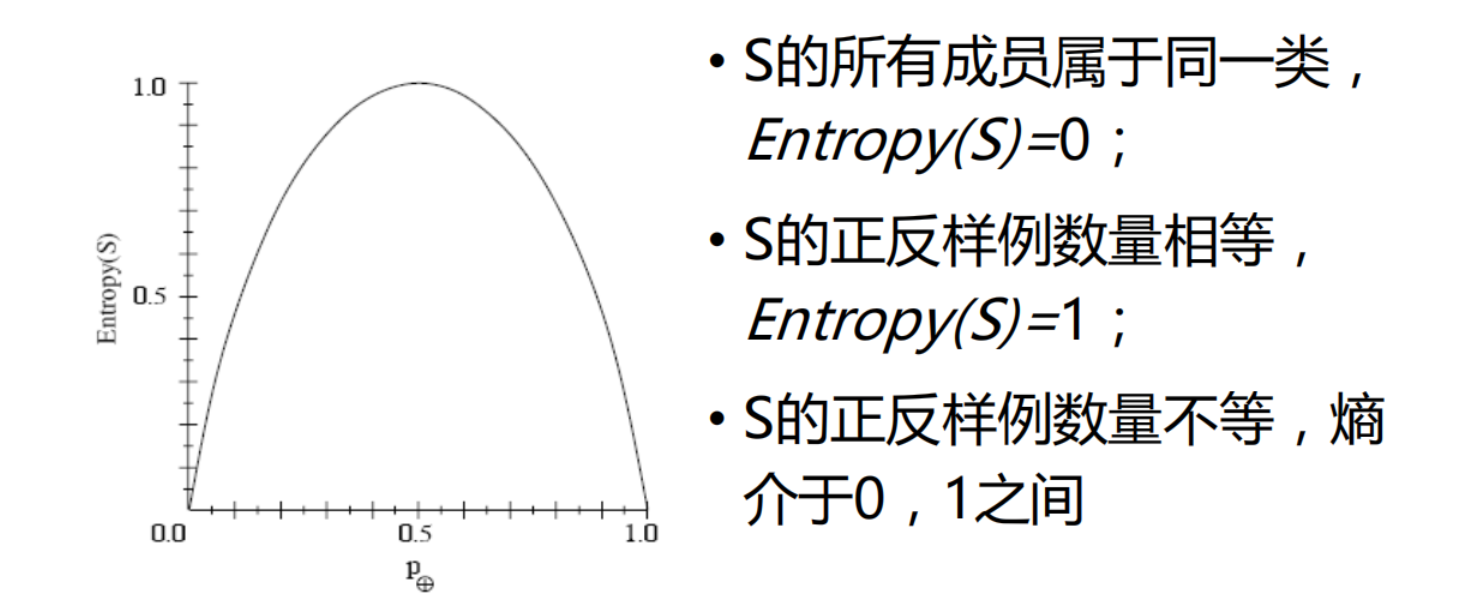
\includegraphics[width=0.5\linewidth]{images/entrofy.png}
        \caption{交叉熵大小含义}
        \label{fig:placeholder}
    \end{figure}
    \item \textbf{条件熵：}对于在 $\mathrm{X}$ 的条件下 $\mathrm{Y}$ 的条件熵,是指在 $\mathrm{X}$ 的信息之后, $\mathrm{Y}$ 这个变量的信息量(不确定性)的大小，计算公式如下：
    $$\operatorname{Entropy}\left( {Y \mid  X}\right)  = \mathop{\sum }\limits_{{i = 1}}^{n}p\left( {x}_{i}\right) \operatorname{Entropy}\left( {Y \mid  {x}_{i}}\right)$$
    {\small\kaishu 例如,当只有A类和B类的时候, $p\left( A\right)  = p\left( B\right)  = {0.5}$ ，熵的大小为：
    $$\text{Entropy}=  - \left( {{0.5lo}{g}_{2}\left( {0.5}\right)  + {0.5lo}{g}_{2}\left( {0.5}\right) }\right)  = 1$$
    }
    \item \textbf{信息增益（Information Gain）：}D本身的熵，减去给定A的条件下D的条件熵。表明引入属性 $\mathrm{A}$ 后,原来数据集 $\mathrm{D}$ 的不确定性减少了多少：
    $$ infoGain \left( {D \mid  A}\right)  = \operatorname{Entropy}\left( D\right)  - \operatorname{Entropy}\left( {D \mid  A}\right)$$
    其中 $A = \left\lbrack  {{a}_{1},{a}_{2},\ldots ,{a}_{k}}\right\rbrack$ ,K个值。
    
    \item \textbf{流程：}
    \begin{enumerate}
        \item \textbf{选择根节点：}使用统计测试确定每一个实例属性单独分类训练样例的能力，分类能力最好的属性被选作树的根节点；
        \item \textbf{排列分支：}为根节点属性的每个可能值产生一个分支，并把训练样例排列到适当的分支；
        \item \textbf{重复上面的过程}：重复上面的过程，用每个分支节点关联的训练样例来选取在该点被测试的最佳属性，直到满足以下两个条件中的任一个：
        \begin{itemize}
            \item 所有的属性已经被这条路径包括\footnote{这个其实是被动停止，因为已经没有属性可以用来分类了，开摆。}；
            \item 与这个节点关联的所有训练样例具有相同的目标属性值\footnote{这个其实是主动停止，因为已经分类干净了，所有的样例都是同样的属性值。}
        \end{itemize}
    \end{enumerate}
    {\small\kaishu
    \begin{figure}[H]
        \centering
        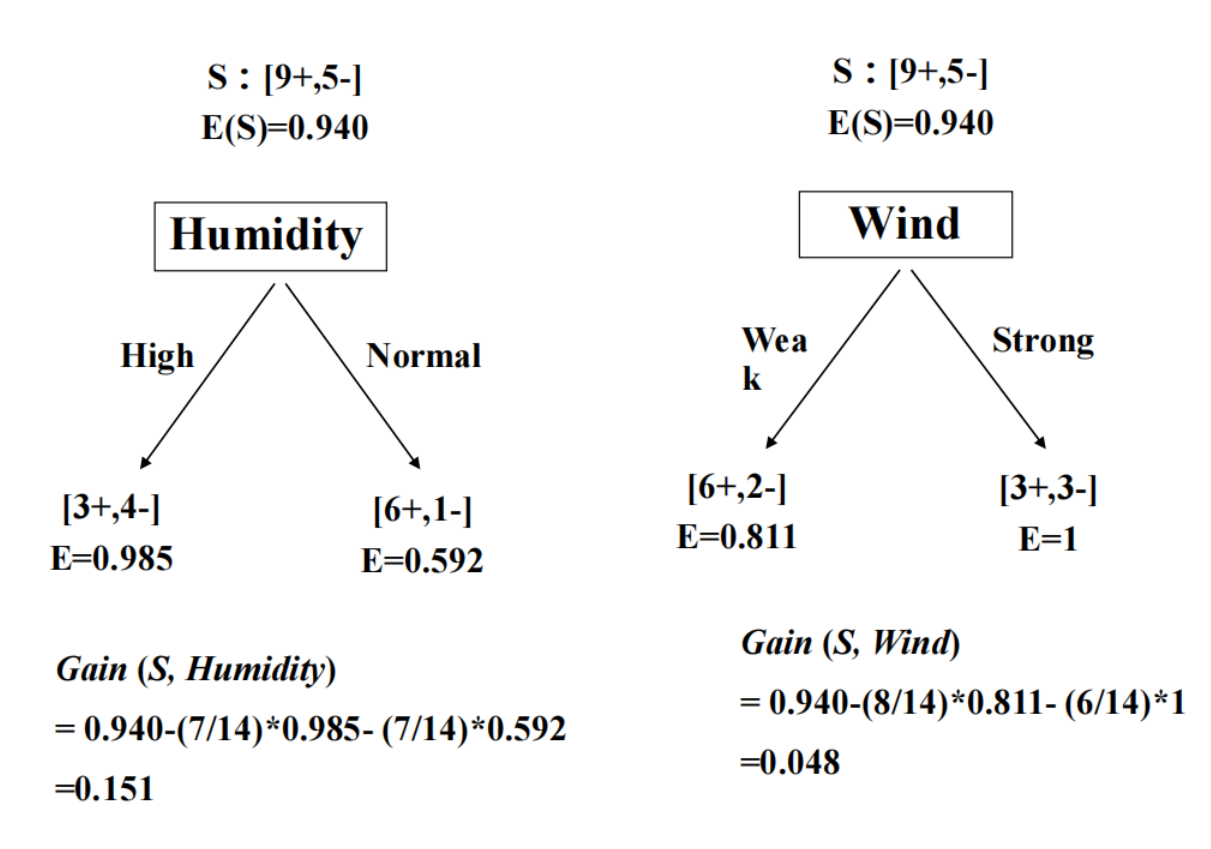
\includegraphics[width=0.55\linewidth]{images/example_entrophy.png}
        \caption{Enter Caption}
        \label{fig:placeholder}
    \end{figure}
    \textbf{例子理解：}以上图中的训练集 $S=[9+,5-]$ 为例，即一开始有9个正例，5个负例，因此正例概率为 $\frac{9}{14}$，负例概率为 $\frac{5}{14}$。由熵的计算公式可得，初始熵为
    $$
    E(S)= - \frac{9}{14}\log_{2}\frac{9}{14} - \frac{5}{14}\log_{2}\frac{5}{14}
    \approx 0.940
    $$
    表示当前样本中正反例混杂，仍然具有较大的不确定性。现在比较两个候选属性：Humidity 和 Wind，目标是看按哪个属性划分后，样本会变得更纯，即信息熵更低。
    
    \begin{enumerate}
        \item \textbf{按 Humidity 划分：}
        可分为两个子集：
        \begin{itemize}
            \item High：$[3+,4-]$，熵为 $0.985$
            \item Normal：$[6+,1-]$，熵为 $0.592$
        \end{itemize}
        划分后的条件熵为
        $$
        E(S\mid \text{Humidity})=\frac{7}{14}\times 0.985+\frac{7}{14}\times 0.592
        $$
        因此信息增益为
        $$
        Gain(S,\text{Humidity})=0.940-\frac{7}{14}\times 0.985-\frac{7}{14}\times 0.592=0.151
        $$
    
        \item \textbf{按 Wind 划分：}
        可分为两个子集：
        \begin{itemize}
            \item Weak：$[6+,2-]$，熵为 $0.811$
            \item Strong：$[3+,3-]$，熵为 $1$
        \end{itemize}
        划分后的条件熵为
        $$
        E(S\mid \text{Wind})=\frac{8}{14}\times 0.811+\frac{6}{14}\times 1
        $$
        因此信息增益为
        $$
        Gain(S,\text{Wind})=0.940-\frac{8}{14}\times 0.811-\frac{6}{14}\times 1=0.048
        $$
    
        \item \textbf{结果比较：}
        $$
        Gain(S,\text{Humidity})=0.151 > Gain(S,\text{Wind})=0.048
        $$
        因此说明 \textbf{Humidity 划分后，不确定性下降得更多，分类效果更好}，所以 ID3 会优先选择 \textbf{Humidity} 作为当前节点的划分属性。之后，因为Humidity这个属性有High和Normal两类取值，分别有7个实例，在此基础上再选择新的属性使得信息增益最高再继续往下分...子子孙孙无穷匮也。
    \end{enumerate}
    }
\end{enumerate}
\subsection{假设空间和归纳偏置}
是指决策树学习的假设空间和归纳偏置。
\begin{enumerate}
    \item \textbf{假设空间：}ID3算法搜索的假设空间就是可能的决策树的集合。
    \item \textbf{搜索策略：}ID3以爬山算法遍历这个假设空间，引导这种爬山搜索的评估函数是信息增益度量。
    {\small\kaishu
    \begin{itemize}
        \item 假设空间包括所有可能的决策树，也就是现有属性能表示出来的全部分类情况；
        \item 每次只保留当前选中的这一棵树，无法知道还有多少棵树也能符合训练数据；
        \item 搜索过程中不会回头修改前面的选择，因此可能只找到局部最优解；
        \item 每一步都是根据当前节点的全部训练样例来选属性，因此比只看单个样例更不容易出错。
    \end{itemize}
    }
    \item \textbf{归纳偏置：}近似的归纳偏置：较短的树比起较长的树优先，信息增益高的属性更靠近根节点的树优先\footnote{很难准确刻画ID3的归纳偏置，只能近似}。

    \item \textbf{限定偏置和优选偏置：}
    \begin{itemize}
        \item 优选偏置（搜索偏置）：ID3的归纳偏置是对某种假设胜过其他假设的一种优选，对最终可列举的假设没有硬性限制\footnote{是通过搜索时的规则偏向某些树：优先选信息增益高的属性优先让高增益属性靠近根通常更容易得到较短的树贪婪、局部地构造树；通常优选偏置比限定偏置更符合归纳学习的需要}；
        \item 限定偏置（语言偏置）：候选消除算法的偏置是对待考虑假设的一种限定；
    \end{itemize}

    \item \textbf{ID3和候选消除算法的比较：}
    \begin{table}[H]
        \centering
        \caption{ID3和候选消除算法的比较}
        \begin{tabular}{p{3.2cm}p{5.6cm}p{5.6cm}}
            \toprule
            比较项目 & ID3 & 候选消除算法 \\
            \midrule
            搜索范围 & 搜索范围是一个完整的假设空间，但不彻底地搜索这个空间 & 搜索范围是不完整的假设空间，但彻底地搜索这个空间 \\
            \midrule
            归纳偏置\footnote{回顾：归纳偏置是指，当多个假设都能解释训练数据时，学习算法为什么会更偏向其中某一些假设。}来源 & 归纳偏置完全是搜索策略排序假设的结果，来自搜索策略 & 完全是假设表示的表达能力的结果，来自对搜索空间的定义 \\
            \bottomrule
        \end{tabular}
    \end{table}

    \item \textbf{为什么短的假设优先：}
    \begin{itemize}
        \item 奥坎姆剃刀：优先选择拟合数据的最简单的假设；
        \item \textbf{原因}：因为简单假设的数量远比复杂假设的数量少，简单假设对训练样例的针对性更小，更像是泛化的规律，而不是训练样例的另一种描述。
    \end{itemize}

    \item \textbf{决策树学习的常见问题：}
    \begin{itemize}
        \item 如何控制决策树的深度；
        \item 如何处理连续值属性；
        \item 如何选择合适的属性选择标准；
        \item 如何处理属性值缺失的训练数据；
        \item 如何处理代价不同的属性；
        \item 如何提高计算效率。
    \end{itemize}
    针对这些问题，ID3 被进一步扩展为 C4.5。
\end{enumerate}
\subsection{过拟合}
\begin{enumerate}
    \item \textbf{原因：}
    \begin{enumerate}
        \item 训练样例含有随机错误或噪声
        \item 即使训练数据无噪声，样本过少时也可能学到偶然规律
    \end{enumerate}
    \item \textbf{结果：}过度拟合使决策树的精度降低10\%到25\%
    \item \textbf{解决办法：}\textbf{预剪枝}和\textbf{后剪枝}
    \begin{itemize}
        \item 及早停止树增长（更直观，但精确地估计何时停止树增长很困难）；
        \item 后修剪法（实践中更成功）；
        \item 训练和验证集法（常见做法是样例的三分之二作训练集合，三分之一作验证集合）；
        \item 错误率降低修剪（直接在树上剪）：将树上的每一个节点作为修剪候选对象，删除以该节点为根的子树，使它成为叶结点，并把与该节点关联的训练样例的最常见分类赋给它；反复选择那些删除后可最大提高决策树在验证集合上精度的节点进行修剪，直到进一步修剪有害为止；
        \item 规则后修剪（先把树变成规则，再对每条规则单独剪）：先从训练集合推导出决策树，使其尽可能拟合训练数据，再将决策树转化为等价规则集，通过删除不会导致估计精度降低的前件来修剪每条规则，并按修剪后规则的估计精度排序后用于分类。
    \end{itemize}
\end{enumerate}

\subsection{ID3算法的扩展}
\begin{enumerate}
    \item \textbf{原因：}
    \begin{itemize}
        \item ID3 只能处理离散值属性；
        \item 信息增益对取值较多的属性有偏置；
        \item 现实数据中可能存在属性值缺失；
        \item 不同属性可能具有不同代价；
        \item 还需要进一步提高计算效率。
    \end{itemize}

    \item \textbf{主要扩展：}
    \begin{itemize}
        \item 处理连续值属性：将连续属性按阈值离散化；
        \item 改进属性选择标准：采用增益率、距离等度量；
        \item 处理缺失属性值：用最常见值或概率方式估计；
        \item 处理不同代价的属性：在属性选择时引入代价项。
    \end{itemize}

    \item \textbf{结果：}针对这些问题，ID3 被进一步扩展为 C4.5。
\end{enumerate}
\begin{table}[H]
\centering
\caption{分类树与回归树对比}
\begin{tabular}{p{2.6cm}p{5.2cm}p{5.2cm}}
\toprule
\textbf{对比维度} & \textbf{分类树} & \textbf{回归树} \\
\midrule
目标变量类型 & 离散类别变量 & 连续数值变量 \\
划分目标 & 使子节点类别尽可能纯 & 使子节点内部数值尽可能接近 \\
常用划分标准 & 信息增益、信息增益率、基尼指数 & 平方误差最小、方差最小、残差平方和最小 \\
叶节点输出 & 叶节点中样本数最多的类别（多数类） & 叶节点中样本目标值的均值 \\
对应优化思想 & 降低类别不确定性，提高节点纯度 & 降低节点内数值离散程度，减小预测误差 \\
典型任务 & 邮件分类、疾病诊断、是否批准贷款 & 房价预测、销量预测、温度预测 \\
\bottomrule
\end{tabular}
\end{table}

\end{document}